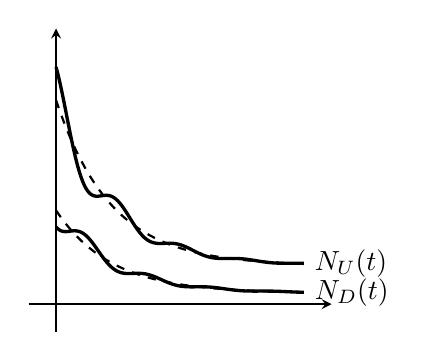
\begin{tikzpicture}[samples=200, scale=.7]
    \coordinate(O)at(0,0);
    \draw[->,>=stealth,semithick](-.5,0)--(5,0);
    \draw[->,>=stealth,semithick](0,-.5)--(0,5);
    \draw[very thick, domain=0:4.5]
    plot(\x,{3*(1+.2*cos(2*pi*50*\x))*exp(-\x)+.7})
    node[anchor=west]{$N_U(t)$}
    ;
    \draw[thick, dashed, domain=0:4.5]
    plot(\x,{3*exp(-\x)+.7})
    ;
    \draw[very thick, domain=0:4.5]
    plot(\x,{1.5*(1-.2*cos(2*pi*50*\x))*exp(-\x)+.2})
    node[anchor=west]{$N_D(t)$}
    ;
    \draw[thick, dashed, domain=0:4.5]
    plot(\x,{1.5*exp(-\x)+.2})
    ;
\end{tikzpicture}
